\documentclass[10pt,a4paper]{article}

\usepackage[top=1.8cm, bottom=1.8cm, left=1.8cm, right=1.8cm]{geometry}
\usepackage[utf8]{inputenc}
\usepackage[portuguese]{babel}
\usepackage{amsmath, amssymb}
\usepackage{booktabs}
\usepackage{graphicx}
\graphicspath{{../}}
\usepackage{microtype}
\usepackage{float}
\usepackage{hyperref}
\usepackage{titlesec}

\titleformat{\section}{\normalsize\bfseries}{\thesection.}{0.5em}{}
\titleformat{\subsection}{\small\bfseries}{\thesubsection.}{0.5em}{}
\titlespacing*{\section}{0pt}{6pt}{3pt}
\titlespacing*{\subsection}{0pt}{4pt}{2pt}

\title{\large\textbf{Relatório Técnico: Heurística Construtiva e Meta-heurística GRASP para o Caminho Hamiltoniano Mínimo}}
\author{Tailan de Souza Oliveira \quad Rubens Rabelo Soares \\
\small Curso de Sistemas de Informação -- Universidade Federal do Ceará (Campus Quixadá) \\
\small Disciplina: Pesquisa Operacional -- Prof. Dr. Paulo Henrique Macêdo}
\date{Outubro de 2026}

\begin{document}

\maketitle
\vspace{-1.8em}

\section{Metodologia e Funcionamento dos Algoritmos}
Este trabalho resolve o Problema do Caminho Hamiltoniano Mínimo (PCHM) em grafos direcionados com origem fixa no vértice $s = 1$ e destino fixo no vértice $t = n$. Os testes foram realizados em Julia 1.12.6 em um computador Linux x86\_64 (Intel Core i5-12450HX com 12 threads e 15,34 GB de RAM DDR5), usando semente fixa (\texttt{seed = 42}) para garantir que os resultados possam ser reproduzidos.

Na Atividade 1, foi implementada a heurística construtiva inicial baseada na regra do vizinho mais próximo. O algoritmo começa no vértice $1$ e, a cada passo, escolhe o vértice intermediário ainda não visitado que possui a viagem mais barata a partir do ponto atual. Quando todos os nós intermediários já foram visitados, o algoritmo liga o último vértice diretamente ao destino final $n$. Por olhar apenas para o próximo passo imediato, essa abordagem é muito rápida, mas costuma deixar conexões caras para o final do caminho.

Na Atividade 2, foi implementada a meta-heurística GRASP com $1000$ iterações e fator de aleatoriedade $\alpha = 0,15$. Em cada iteração, o algoritmo primeiro constrói um caminho escolhendo arestas de forma sorteada dentro de uma Lista Restrita de Candidatos (LRC), que reúne apenas as arestas mais baratas que não violam os graus dos nós nem formam ciclos antes da hora. Para verificar se uma nova aresta fecharia um ciclo indevido, testamos duas formas: uma usando a estrutura de conjuntos disjuntos (\textit{Union-Find}) e outra percorrendo os nós diretamente. Depois de construir o caminho, o algoritmo aplica a busca local VND (\textit{Variable Neighborhood Descent}), que tenta melhorar a rota testando três tipos de modificações nos nós intermediários: o 2-Opt (que inverte um trecho da rota), o Or-Opt (que move blocos de 1, 2 ou 3 nós seguidos para outra posição) e o Swap (que troca dois nós de lugar). Para ganhar velocidade, a busca local calcula apenas a diferença de custo das arestas que mudaram de posição, sem precisar somar a rota inteira novamente.

\section{Resultados Computacionais e Comparação com o Modelo PLI}
A Tabela~\ref{tab:comparacao} reúne os custos e os tempos de execução das 13 instâncias da TSPLIB obtidos pela Heurística Inicial, pelo GRASP (com e sem \textit{Union-Find}) e pelo modelo exato de Programação Linear Inteira (PLI com Gurobi do Trabalho Prático 01, limitado a 180s). A coluna Melhoria mostra quanto o GRASP reduziu o custo em relação à Heurística Inicial ($\frac{Z_{\text{Inicial}} - Z_{\text{GRASP}}}{Z_{\text{Inicial}}} \times 100\%$), enquanto a coluna $\text{Gap}_{\text{PLI}}$ mostra a diferença percentual entre o GRASP e o resultado do modelo exato ($\frac{Z_{\text{GRASP}} - Z_{\text{PLI}}}{Z_{\text{PLI}}} \times 100\%$).

\begin{table}[H]
\centering
\scriptsize
\setlength{\tabcolsep}{3.0pt}
\caption{Comparação entre Heurística Inicial, Meta-heurística GRASP (1000 iterações, $\alpha=0,15$) e Modelo Exato PLI (TP 01).}
\label{tab:comparacao}
\begin{tabular}{lcccccccccc}
\toprule
Instância & $n$ & $Z_{\text{Inicial}}$ & $T_{\text{Inicial}}$ (s) & $Z_{\text{GRASP}}$ & $T_{\text{GRASP}}^{\text{Com UF}}$ (s) & $T_{\text{GRASP}}^{\text{Sem UF}}$ (s) & Melhoria (\%) & $Z_{\text{PLI}}$ (TP1) & $T_{\text{PLI}}$ (s) & $\text{Gap}_{\text{PLI}}$ (\%) \\
\midrule
\texttt{br17.atsp}  & 17 & 56,00    & $< 0,0001$ & 34,00    & 0,2711  & 0,2296  & 39,29\% & 34,00    & 0,32   & 0,00\% \\
\texttt{ft53.atsp}  & 53 & 9583,00  & $< 0,0001$ & 6950,00  & 10,3490 & 11,8697 & 27,48\% & 6196,00  & 12,37  & 12,17\% \\
\texttt{ft70.atsp}  & 70 & 42057,00 & $< 0,0001$ & 39608,00 & 30,6039 & 34,9154 & 5,82\%  & 37655,00 & 2,06   & 5,19\% \\
\texttt{ftv33.atsp} & 34 & 1547,00  & $< 0,0001$ & 1275,00  & 1,3121  & 1,3420  & 17,58\% & 1275,00  & 0,47   & 0,00\% \\
\texttt{ftv35.atsp} & 36 & 1750,00  & $< 0,0001$ & 1455,00  & 1,5804  & 1,7806  & 16,86\% & 1443,00  & 0,35   & 0,83\% \\
\texttt{ftv38.atsp} & 39 & 1828,00  & $< 0,0001$ & 1520,00  & 2,2062  & 2,4271  & 16,85\% & 1511,00  & 0,39   & 0,60\% \\
\texttt{ftv44.atsp} & 45 & 1933,00  & $< 0,0001$ & 1654,00  & 3,8957  & 4,4952  & 14,43\% & 1614,00  & 0,95   & 2,48\% \\
\texttt{ftv47.atsp} & 48 & 2298,00  & $< 0,0001$ & 1796,00  & 5,5489  & 5,8328  & 21,85\% & 1754,00  & 1,43   & 2,39\% \\
\texttt{ftv55.atsp} & 56 & 2052,00  & $< 0,0001$ & 1696,00  & 9,3377  & 10,1509 & 17,35\% & 1613,00  & 2,06   & 5,15\% \\
\texttt{ftv64.atsp} & 65 & 2586,00  & $< 0,0001$ & 1975,00  & 24,8442 & 27,1173 & 23,63\% & 1840,00  & 6,11   & 7,34\% \\
\texttt{ftv70.atsp} & 71 & 2637,00  & $< 0,0001$ & 2104,00  & 34,0494 & 37,3969 & 20,21\% & 1958,00  & 6,89   & 7,46\% \\
\texttt{p43.atsp}   & 43 & 642,00   & $< 0,0001$ & 596,00   & 5,6638  & 5,5128  & 7,17\%  & 589,00*  & 180,04 & 1,19\% \\
\texttt{ry48p.atsp} & 48 & 17971,00 & $< 0,0001$ & 14231,00 & 7,9283  & 7,7672  & 20,81\% & 14070,00 & 1,70   & 1,14\% \\
\bottomrule
\multicolumn{11}{l}{\tiny *Em \texttt{p43.atsp}, o modelo PLI atingiu o tempo limite de 180s sem provar otimalidade global, retornando a melhor solução encontrada ($589,00$).}
\end{tabular}
\end{table}

\section{Análise dos Resultados e Principais Diferenças}
Na comparação entre a Heurística Inicial e o GRASP, a principal diferença aparece na qualidade das rotas geradas. Embora a heurística inicial termine quase instantaneamente (menos de $0,0001\text{ s}$ em todos os testes), ela toma decisões ruins no final do percurso por escolher sempre a aresta mais barata do momento sem planejar a chegada ao destino $n$. O GRASP conseguiu melhorar o resultado inicial em todas as 13 instâncias, com uma redução média de custo de $19,18\%$. As maiores diferenças de custo entre os dois métodos ocorreram em \texttt{br17.atsp}, onde o custo caiu de $56,00$ para $34,00$ (economia de $39,29\%$), em \texttt{ft53.atsp}, onde caiu de $9583,00$ para $6950,00$ (economia de $27,48\%$), e em \texttt{ftv64.atsp}, com redução de $23,63\%$. Mesmo nas instâncias onde a heurística inicial já partia de um valor mais próximo, como \texttt{ft70.atsp} e \texttt{p43.atsp}, o GRASP ainda reduziu o custo em $5,82\%$ e $7,17\%$, respectivamente.

Quando comparamos o GRASP com o modelo exato de Programação Linear Inteira (PLI) do Trabalho Prático 01, observamos que o GRASP encontrou exatamente a solução ótima ($\text{Gap}_{\text{PLI}} = 0,00\%$) em \texttt{br17.atsp} ($34,00$) e \texttt{ftv33.atsp} ($1275,00$), além de ficar muito próximo do ótimo (diferença abaixo de $2,50\%$) em outras seis instâncias: \texttt{ftv38.atsp} ($0,60\%$), \texttt{ftv35.atsp} ($0,83\%$), \texttt{ry48p.atsp} ($1,14\%$), \texttt{p43.atsp} ($1,19\%$), \texttt{ftv47.atsp} ($2,39\%$) e \texttt{ftv44.atsp} ($2,48\%$). A maior diferença de qualidade a favor do PLI ocorreu em \texttt{ft53.atsp}, na qual o GRASP ficou $12,17\%$ acima do ótimo exato ($6950,00$ contra $6196,00$), seguida pelas instâncias maiores \texttt{ftv70.atsp} ($7,46\%$) e \texttt{ftv64.atsp} ($7,34\%$), onde o espaço de busca cresce muito para $1000$ iterações.

Em relação ao tempo de execução entre GRASP e PLI, a maior diferença a favor do GRASP aconteceu na instância \texttt{p43.atsp}: enquanto o solver exato Gurobi travou na árvore de busca e atingiu o tempo máximo de $180,04\text{ s}$, o GRASP entregou uma solução apenas $1,19\%$ acima em $5,66\text{ s}$, sendo mais de $31$ vezes mais rápido. Na instância \texttt{ft53.atsp}, o GRASP também terminou em tempo menor que o PLI ($10,35\text{ s}$ contra $12,37\text{ s}$). Por outro lado, a maior diferença de tempo a favor do PLI ocorreu nas instâncias com mais de 60 vértices, especialmente em \texttt{ft70.atsp} e \texttt{ftv70.atsp}, nas quais o Gurobi levou $2,06\text{ s}$ e $6,89\text{ s}$, enquanto o GRASP precisou de $30,60\text{ s}$ e $34,05\text{ s}$ porque a busca local Or-Opt testa combinações na ordem de $O(n^3)$ em cada uma das $1000$ iterações.

Por fim, comparando as duas versões do GRASP (com e sem \textit{Union-Find}), ambas chegaram exatamente aos mesmos custos finais por usarem a mesma semente aleatória, mas o tempo de execução mostrou diferenças importantes conforme o grafo cresce. Nas instâncias pequenas ou médias como \texttt{br17.atsp} e \texttt{p43.atsp}, a versão sem \textit{Union-Find} teve tempo praticamente igual ou frações de segundo menor devido à simplicidade de percorrer poucos nós. Já nas maiores instâncias, o \textit{Union-Find} fez diferença clara no tempo total, economizando $4,31\text{ s}$ em \texttt{ft70.atsp} ($12,3\%$ mais rápido), $3,35\text{ s}$ em \texttt{ftv70.atsp} ($9,0\%$ mais rápido), $2,27\text{ s}$ em \texttt{ftv64.atsp} ($8,4\%$ mais rápido) e $1,52\text{ s}$ em \texttt{ft53.atsp} ($12,8\%$ mais rápido).

\section{Rotas Encontradas pela Meta-heurística GRASP}
\small
\noindent \textbf{br17 (34,00):} 1 $\to$ 12 $\to$ 3 $\to$ 14 $\to$ 2 $\to$ 13 $\to$ 11 $\to$ 10 $\to$ 15 $\to$ 7 $\to$ 6 $\to$ 16 $\to$ 5 $\to$ 4 $\to$ 8 $\to$ 9 $\to$ 17. \\
\textbf{ft53 (6950,00):} 1 $\to$ 37 $\to$ 33 $\to$ 34 $\to$ 27 $\to$ 26 $\to$ 28 $\to$ 30 $\to$ 29 $\to$ 32 $\to$ 31 $\to$ 5 $\to$ 3 $\to$ 16 $\to$ 38 $\to$ 36 $\to$ 41 $\to$ 40 $\to$ 39 $\to$ 46 $\to$ 43 $\to$ 47 $\to$ 44 $\to$ 42 $\to$ 48 $\to$ 45 $\to$ 35 $\to$ 19 $\to$ 18 $\to$ 17 $\to$ 24 $\to$ 21 $\to$ 22 $\to$ 25 $\to$ 23 $\to$ 20 $\to$ 2 $\to$ 4 $\to$ 12 $\to$ 11 $\to$ 13 $\to$ 15 $\to$ 14 $\to$ 10 $\to$ 9 $\to$ 8 $\to$ 7 $\to$ 6 $\to$ 52 $\to$ 51 $\to$ 49 $\to$ 50 $\to$ 53. \\
\textbf{ft70 (39608,00):} 1 $\to$ 2 $\to$ 61 $\to$ 60 $\to$ 11 $\to$ 15 $\to$ 64 $\to$ 67 $\to$ 65 $\to$ 69 $\to$ 66 $\to$ 68 $\to$ 36 $\to$ 39 $\to$ 14 $\to$ 9 $\to$ 47 $\to$ 46 $\to$ 63 $\to$ 62 $\to$ 59 $\to$ 58 $\to$ 45 $\to$ 49 $\to$ 44 $\to$ 50 $\to$ 48 $\to$ 56 $\to$ 54 $\to$ 24 $\to$ 22 $\to$ 27 $\to$ 3 $\to$ 5 $\to$ 28 $\to$ 23 $\to$ 26 $\to$ 4 $\to$ 6 $\to$ 7 $\to$ 17 $\to$ 16 $\to$ 29 $\to$ 55 $\to$ 53 $\to$ 52 $\to$ 51 $\to$ 19 $\to$ 20 $\to$ 31 $\to$ 35 $\to$ 33 $\to$ 30 $\to$ 13 $\to$ 10 $\to$ 12 $\to$ 8 $\to$ 21 $\to$ 18 $\to$ 25 $\to$ 57 $\to$ 34 $\to$ 32 $\to$ 37 $\to$ 43 $\to$ 42 $\to$ 41 $\to$ 40 $\to$ 38 $\to$ 70. \\
\textbf{ftv33 (1275,00):} 1 $\to$ 2 $\to$ 3 $\to$ 4 $\to$ 14 $\to$ 13 $\to$ 15 $\to$ 16 $\to$ 17 $\to$ 26 $\to$ 25 $\to$ 24 $\to$ 27 $\to$ 28 $\to$ 29 $\to$ 30 $\to$ 23 $\to$ 21 $\to$ 22 $\to$ 32 $\to$ 19 $\to$ 20 $\to$ 18 $\to$ 12 $\to$ 9 $\to$ 11 $\to$ 10 $\to$ 33 $\to$ 8 $\to$ 5 $\to$ 7 $\to$ 6 $\to$ 31 $\to$ 34. \\
\textbf{ftv35 (1455,00):} 1 $\to$ 14 $\to$ 13 $\to$ 6 $\to$ 7 $\to$ 8 $\to$ 35 $\to$ 9 $\to$ 10 $\to$ 12 $\to$ 15 $\to$ 16 $\to$ 17 $\to$ 27 $\to$ 2 $\to$ 4 $\to$ 3 $\to$ 5 $\to$ 33 $\to$ 31 $\to$ 28 $\to$ 24 $\to$ 26 $\to$ 25 $\to$ 18 $\to$ 11 $\to$ 34 $\to$ 19 $\to$ 20 $\to$ 21 $\to$ 22 $\to$ 23 $\to$ 29 $\to$ 30 $\to$ 32 $\to$ 36. \\
\textbf{ftv38 (1520,00):} 1 $\to$ 17 $\to$ 16 $\to$ 9 $\to$ 38 $\to$ 10 $\to$ 11 $\to$ 13 $\to$ 12 $\to$ 15 $\to$ 18 $\to$ 19 $\to$ 20 $\to$ 2 $\to$ 4 $\to$ 3 $\to$ 5 $\to$ 6 $\to$ 8 $\to$ 7 $\to$ 36 $\to$ 34 $\to$ 30 $\to$ 29 $\to$ 28 $\to$ 21 $\to$ 14 $\to$ 37 $\to$ 22 $\to$ 23 $\to$ 24 $\to$ 25 $\to$ 26 $\to$ 27 $\to$ 31 $\to$ 32 $\to$ 33 $\to$ 35 $\to$ 39. \\
\textbf{ftv44 (1654,00):} 1 $\to$ 22 $\to$ 20 $\to$ 15 $\to$ 11 $\to$ 44 $\to$ 12 $\to$ 13 $\to$ 14 $\to$ 16 $\to$ 17 $\to$ 18 $\to$ 19 $\to$ 43 $\to$ 23 $\to$ 24 $\to$ 25 $\to$ 26 $\to$ 27 $\to$ 28 $\to$ 29 $\to$ 31 $\to$ 30 $\to$ 33 $\to$ 34 $\to$ 35 $\to$ 37 $\to$ 38 $\to$ 4 $\to$ 5 $\to$ 6 $\to$ 21 $\to$ 8 $\to$ 10 $\to$ 9 $\to$ 41 $\to$ 42 $\to$ 7 $\to$ 40 $\to$ 39 $\to$ 36 $\to$ 32 $\to$ 2 $\to$ 3 $\to$ 45. \\
\textbf{ftv47 (1796,00):} 1 $\to$ 26 $\to$ 2 $\to$ 10 $\to$ 34 $\to$ 28 $\to$ 4 $\to$ 25 $\to$ 5 $\to$ 30 $\to$ 31 $\to$ 6 $\to$ 32 $\to$ 7 $\to$ 11 $\to$ 9 $\to$ 12 $\to$ 38 $\to$ 19 $\to$ 18 $\to$ 13 $\to$ 33 $\to$ 8 $\to$ 24 $\to$ 35 $\to$ 14 $\to$ 47 $\to$ 37 $\to$ 15 $\to$ 36 $\to$ 16 $\to$ 17 $\to$ 46 $\to$ 21 $\to$ 39 $\to$ 27 $\to$ 43 $\to$ 29 $\to$ 3 $\to$ 42 $\to$ 44 $\to$ 23 $\to$ 20 $\to$ 45 $\to$ 40 $\to$ 22 $\to$ 41 $\to$ 48. \\
\textbf{ftv55 (1696,00):} 1 $\to$ 34 $\to$ 2 $\to$ 4 $\to$ 49 $\to$ 32 $\to$ 47 $\to$ 35 $\to$ 3 $\to$ 15 $\to$ 11 $\to$ 8 $\to$ 33 $\to$ 9 $\to$ 37 $\to$ 10 $\to$ 38 $\to$ 12 $\to$ 52 $\to$ 13 $\to$ 16 $\to$ 17 $\to$ 18 $\to$ 53 $\to$ 27 $\to$ 26 $\to$ 25 $\to$ 43 $\to$ 22 $\to$ 23 $\to$ 42 $\to$ 51 $\to$ 24 $\to$ 55 $\to$ 28 $\to$ 50 $\to$ 30 $\to$ 21 $\to$ 41 $\to$ 20 $\to$ 19 $\to$ 40 $\to$ 39 $\to$ 14 $\to$ 36 $\to$ 5 $\to$ 7 $\to$ 6 $\to$ 48 $\to$ 45 $\to$ 29 $\to$ 54 $\to$ 44 $\to$ 46 $\to$ 31 $\to$ 56. \\
\textbf{ftv64 (1975,00):} 1 $\to$ 16 $\to$ 62 $\to$ 51 $\to$ 29 $\to$ 28 $\to$ 27 $\to$ 23 $\to$ 24 $\to$ 31 $\to$ 54 $\to$ 32 $\to$ 63 $\to$ 53 $\to$ 52 $\to$ 25 $\to$ 26 $\to$ 64 $\to$ 30 $\to$ 33 $\to$ 55 $\to$ 2 $\to$ 38 $\to$ 4 $\to$ 19 $\to$ 18 $\to$ 17 $\to$ 14 $\to$ 47 $\to$ 46 $\to$ 11 $\to$ 61 $\to$ 15 $\to$ 48 $\to$ 8 $\to$ 37 $\to$ 9 $\to$ 41 $\to$ 42 $\to$ 10 $\to$ 43 $\to$ 44 $\to$ 45 $\to$ 12 $\to$ 13 $\to$ 36 $\to$ 20 $\to$ 21 $\to$ 22 $\to$ 49 $\to$ 50 $\to$ 60 $\to$ 56 $\to$ 34 $\to$ 57 $\to$ 39 $\to$ 3 $\to$ 5 $\to$ 40 $\to$ 6 $\to$ 7 $\to$ 58 $\to$ 59 $\to$ 35 $\to$ 65. \\
\textbf{ftv70 (2104,00):} 1 $\to$ 29 $\to$ 26 $\to$ 28 $\to$ 7 $\to$ 14 $\to$ 67 $\to$ 15 $\to$ 13 $\to$ 16 $\to$ 17 $\to$ 19 $\to$ 20 $\to$ 21 $\to$ 22 $\to$ 23 $\to$ 24 $\to$ 61 $\to$ 33 $\to$ 34 $\to$ 70 $\to$ 42 $\to$ 64 $\to$ 41 $\to$ 69 $\to$ 47 $\to$ 63 $\to$ 53 $\to$ 46 $\to$ 54 $\to$ 45 $\to$ 44 $\to$ 43 $\to$ 36 $\to$ 35 $\to$ 37 $\to$ 38 $\to$ 39 $\to$ 40 $\to$ 48 $\to$ 49 $\to$ 52 $\to$ 51 $\to$ 68 $\to$ 50 $\to$ 55 $\to$ 56 $\to$ 4 $\to$ 5 $\to$ 9 $\to$ 8 $\to$ 10 $\to$ 12 $\to$ 11 $\to$ 59 $\to$ 62 $\to$ 60 $\to$ 58 $\to$ 57 $\to$ 6 $\to$ 32 $\to$ 31 $\to$ 30 $\to$ 25 $\to$ 27 $\to$ 18 $\to$ 65 $\to$ 66 $\to$ 2 $\to$ 3 $\to$ 71. \\
\textbf{p43 (596,00):} 1 $\to$ 5 $\to$ 38 $\to$ 7 $\to$ 6 $\to$ 8 $\to$ 12 $\to$ 10 $\to$ 11 $\to$ 9 $\to$ 33 $\to$ 32 $\to$ 30 $\to$ 31 $\to$ 35 $\to$ 34 $\to$ 15 $\to$ 13 $\to$ 14 $\to$ 16 $\to$ 18 $\to$ 17 $\to$ 21 $\to$ 19 $\to$ 20 $\to$ 27 $\to$ 26 $\to$ 25 $\to$ 22 $\to$ 24 $\to$ 23 $\to$ 36 $\to$ 37 $\to$ 3 $\to$ 2 $\to$ 4 $\to$ 29 $\to$ 28 $\to$ 40 $\to$ 39 $\to$ 42 $\to$ 41 $\to$ 43. \\
\textbf{ry48p (14231,00):} 1 $\to$ 9 $\to$ 40 $\to$ 15 $\to$ 12 $\to$ 47 $\to$ 20 $\to$ 33 $\to$ 46 $\to$ 36 $\to$ 7 $\to$ 18 $\to$ 28 $\to$ 30 $\to$ 37 $\to$ 43 $\to$ 17 $\to$ 27 $\to$ 19 $\to$ 6 $\to$ 44 $\to$ 31 $\to$ 38 $\to$ 8 $\to$ 16 $\to$ 22 $\to$ 3 $\to$ 41 $\to$ 34 $\to$ 11 $\to$ 23 $\to$ 14 $\to$ 25 $\to$ 13 $\to$ 21 $\to$ 39 $\to$ 32 $\to$ 24 $\to$ 10 $\to$ 45 $\to$ 35 $\to$ 4 $\to$ 26 $\to$ 42 $\to$ 2 $\to$ 29 $\to$ 5 $\to$ 48.
\normalsize

\section{Representação Gráfica das Rotas (GRASP)}
As Figuras~\ref{fig:br17} a~\ref{fig:ftv70} exibem o mapeamento bidimensional das rotas geradas pelo GRASP nas 13 instâncias da TSPLIB, destacando a transição contínua da origem ($s=1$, verde) ao destino ($t=n$, vermelho).

\begin{figure}[H]
\centering
\begin{minipage}{0.48\textwidth}
\centering
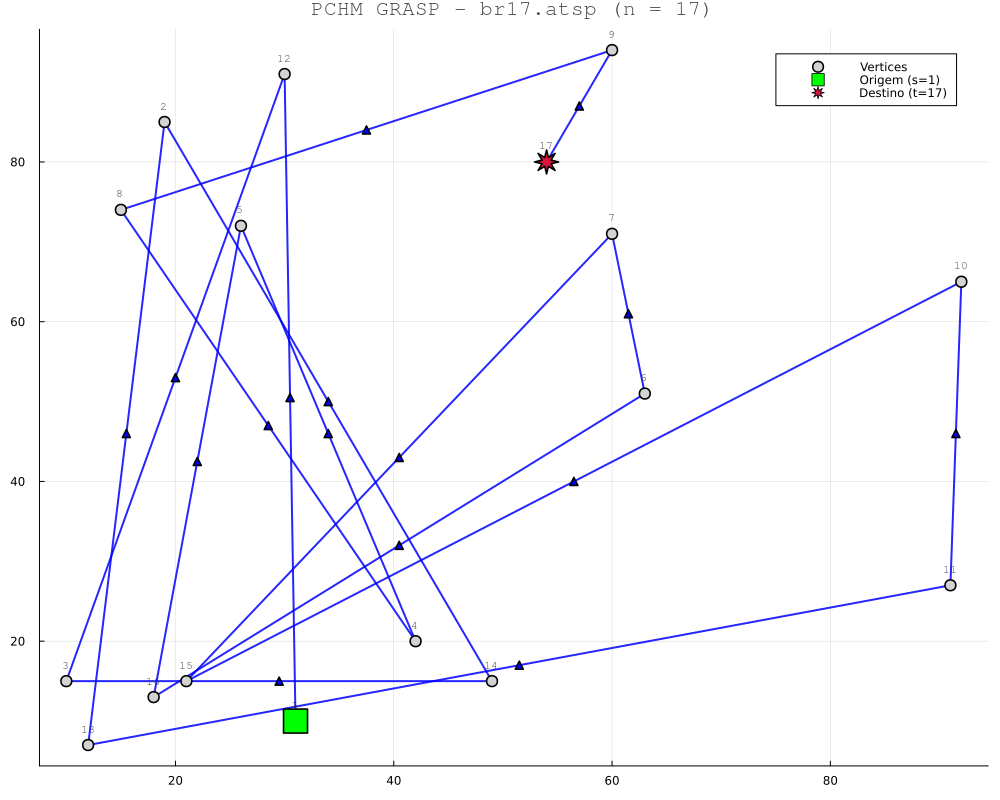
\includegraphics[width=\linewidth]{data/plots/br17.png}
\caption{\texttt{br17.atsp} ($n=17$, $Z_{\text{GRASP}} = 34,00$)}\label{fig:br17}
\end{minipage}
\hfill
\begin{minipage}{0.48\textwidth}
\centering
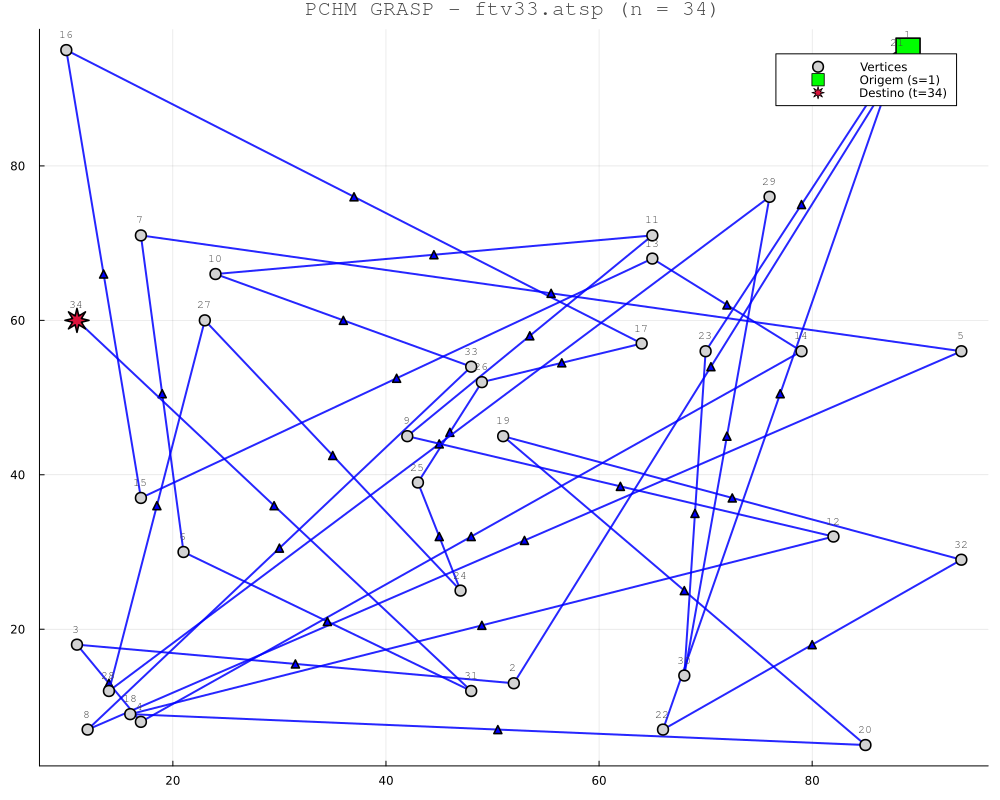
\includegraphics[width=\linewidth]{data/plots/ftv33.png}
\caption{\texttt{ftv33.atsp} ($n=34$, $Z_{\text{GRASP}} = 1275,00$)}
\end{minipage}
\end{figure}

\begin{figure}[H]
\centering
\begin{minipage}{0.48\textwidth}
\centering
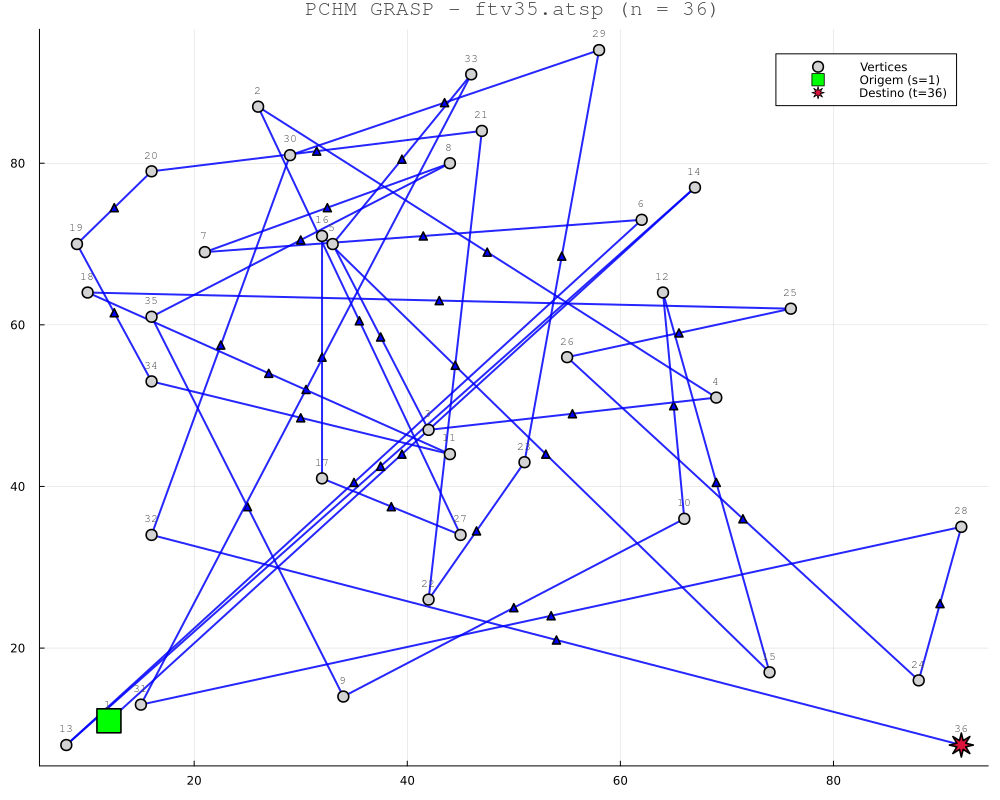
\includegraphics[width=\linewidth]{data/plots/ftv35.png}
\caption{\texttt{ftv35.atsp} ($n=36$, $Z_{\text{GRASP}} = 1455,00$)}
\end{minipage}
\hfill
\begin{minipage}{0.48\textwidth}
\centering
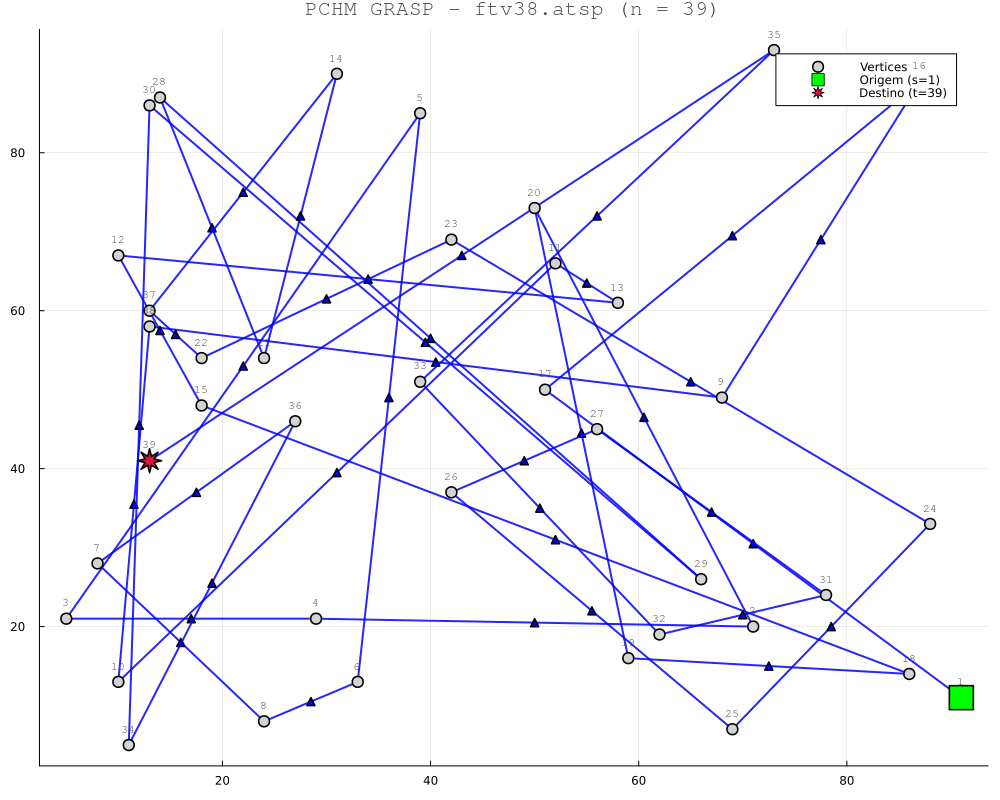
\includegraphics[width=\linewidth]{data/plots/ftv38.png}
\caption{\texttt{ftv38.atsp} ($n=39$, $Z_{\text{GRASP}} = 1520,00$)}
\end{minipage}
\end{figure}

\begin{figure}[H]
\centering
\begin{minipage}{0.48\textwidth}
\centering
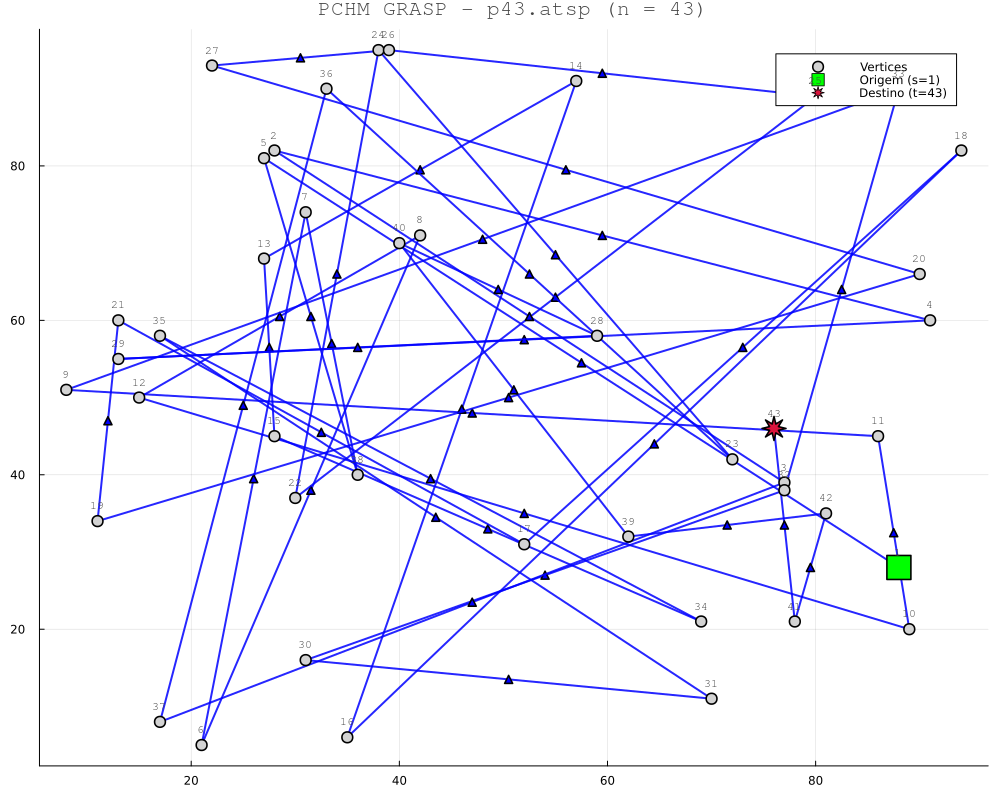
\includegraphics[width=\linewidth]{data/plots/p43.png}
\caption{\texttt{p43.atsp} ($n=43$, $Z_{\text{GRASP}} = 596,00$)}
\end{minipage}
\hfill
\begin{minipage}{0.48\textwidth}
\centering
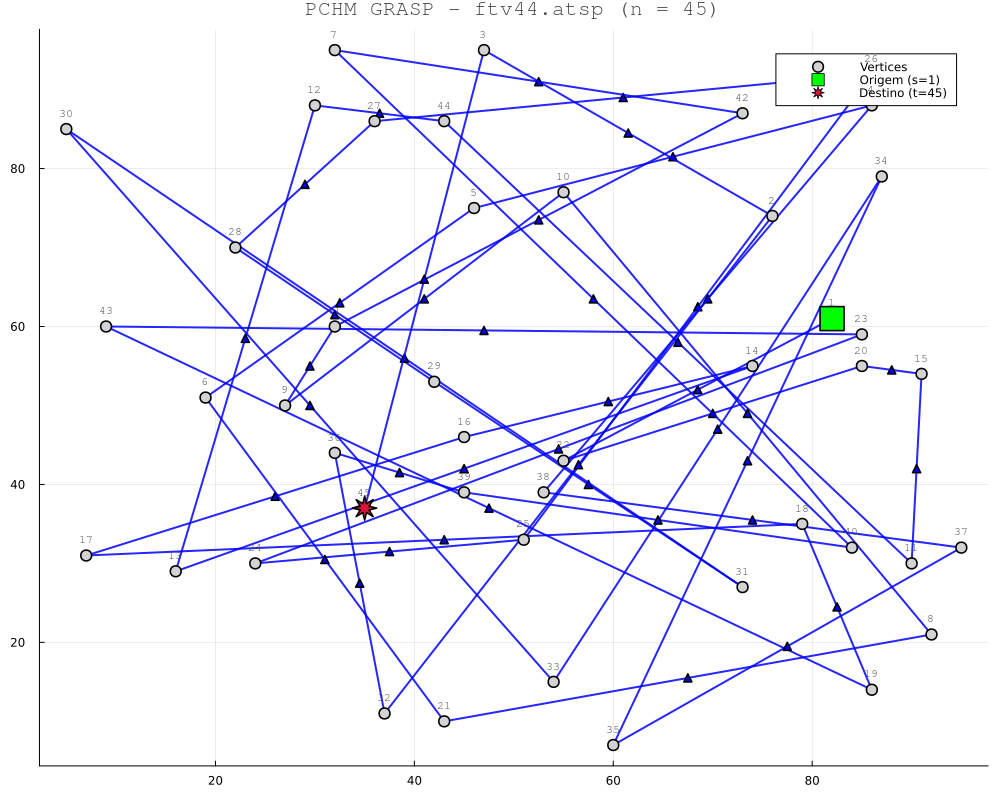
\includegraphics[width=\linewidth]{data/plots/ftv44.png}
\caption{\texttt{ftv44.atsp} ($n=45$, $Z_{\text{GRASP}} = 1654,00$)}
\end{minipage}
\end{figure}

\begin{figure}[H]
\centering
\begin{minipage}{0.48\textwidth}
\centering
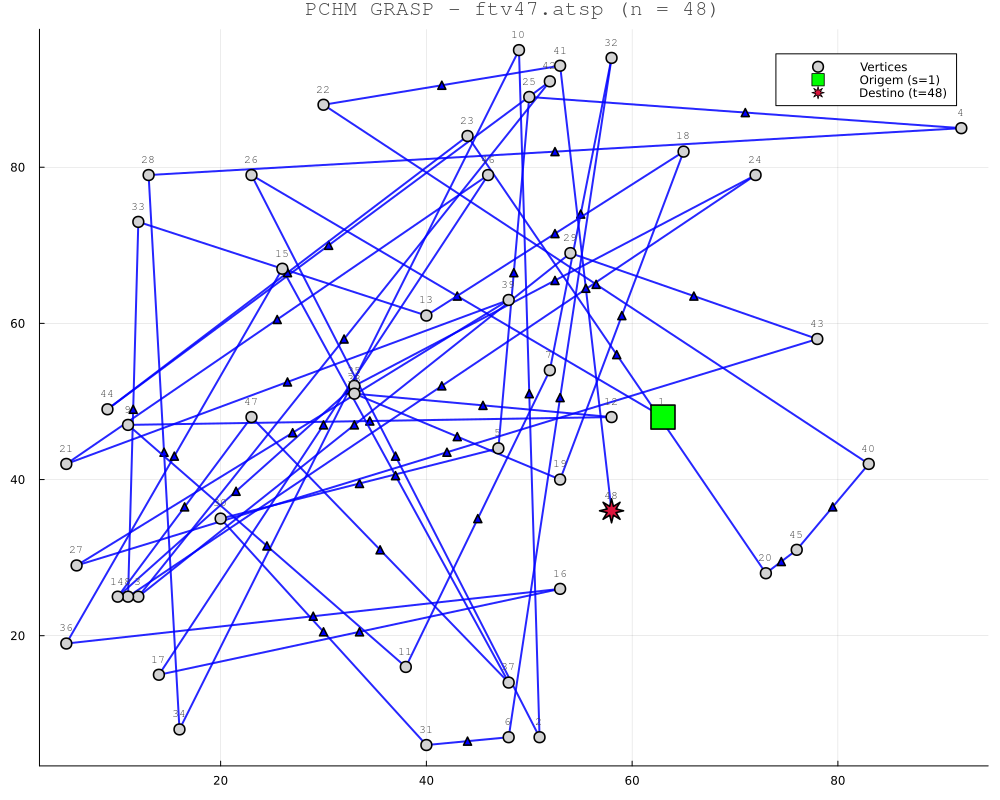
\includegraphics[width=\linewidth]{data/plots/ftv47.png}
\caption{\texttt{ftv47.atsp} ($n=48$, $Z_{\text{GRASP}} = 1796,00$)}
\end{minipage}
\hfill
\begin{minipage}{0.48\textwidth}
\centering
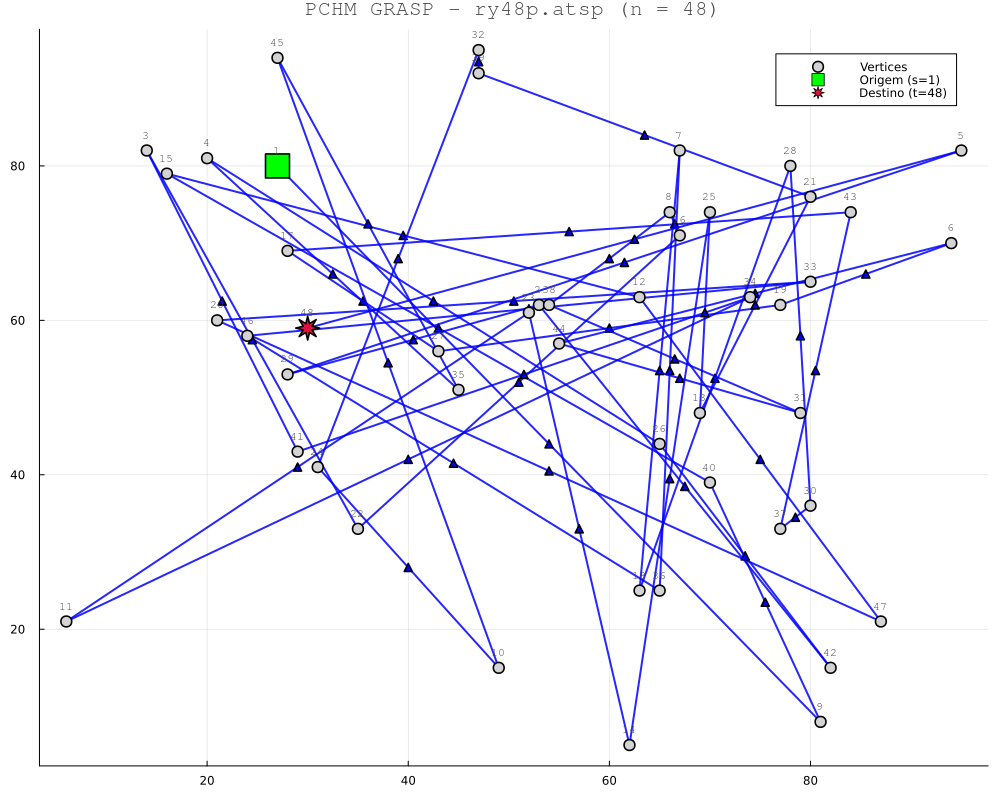
\includegraphics[width=\linewidth]{data/plots/ry48p.png}
\caption{\texttt{ry48p.atsp} ($n=48$, $Z_{\text{GRASP}} = 14231,00$)}
\end{minipage}
\end{figure}

\begin{figure}[H]
\centering
\begin{minipage}{0.48\textwidth}
\centering
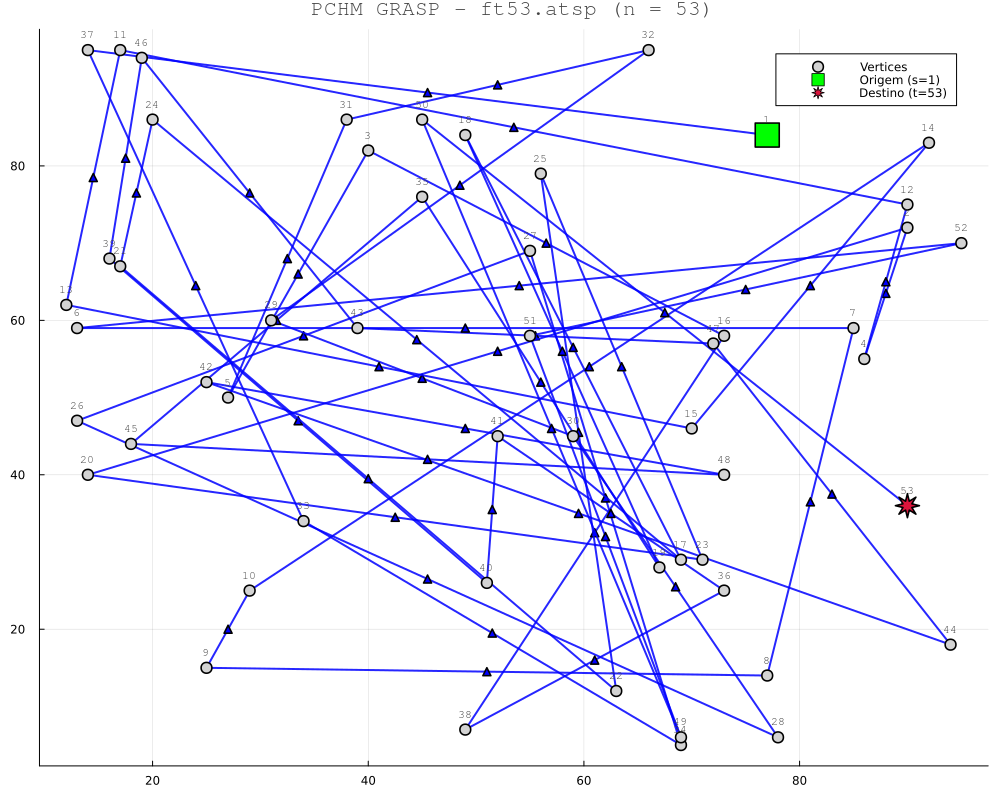
\includegraphics[width=\linewidth]{data/plots/ft53.png}
\caption{\texttt{ft53.atsp} ($n=53$, $Z_{\text{GRASP}} = 6950,00$)}
\end{minipage}
\hfill
\begin{minipage}{0.48\textwidth}
\centering
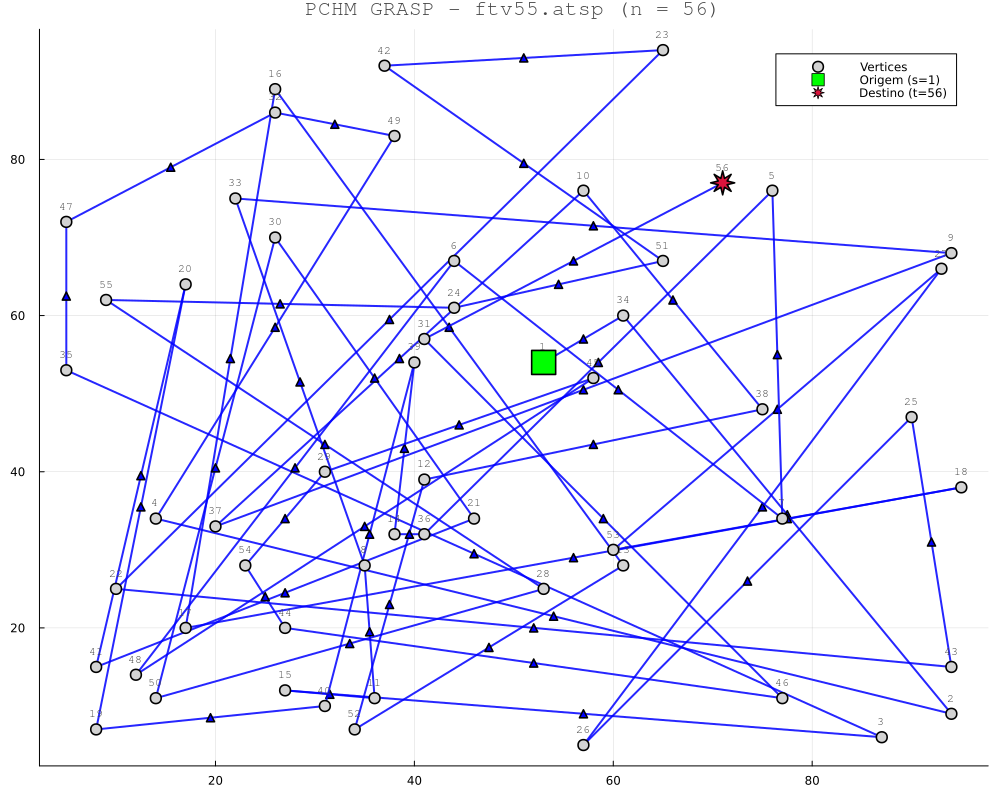
\includegraphics[width=\linewidth]{data/plots/ftv55.png}
\caption{\texttt{ftv55.atsp} ($n=56$, $Z_{\text{GRASP}} = 1696,00$)}
\end{minipage}
\end{figure}

\begin{figure}[H]
\centering
\begin{minipage}{0.48\textwidth}
\centering
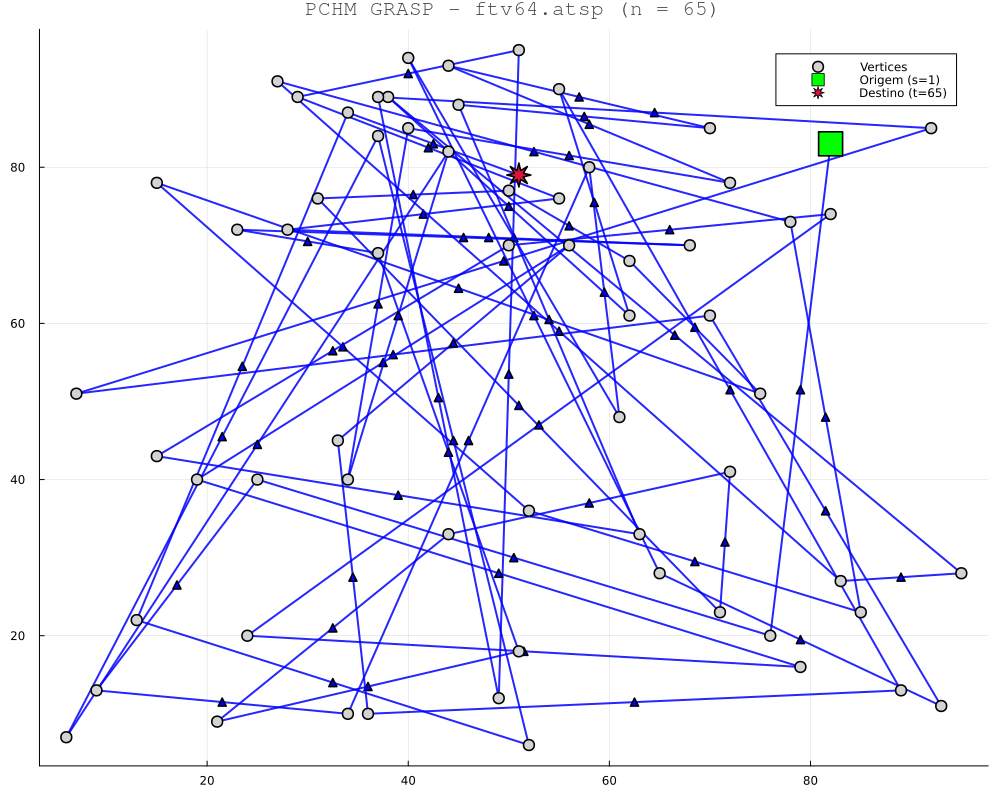
\includegraphics[width=\linewidth]{data/plots/ftv64.png}
\caption{\texttt{ftv64.atsp} ($n=65$, $Z_{\text{GRASP}} = 1975,00$)}
\end{minipage}
\hfill
\begin{minipage}{0.48\textwidth}
\centering
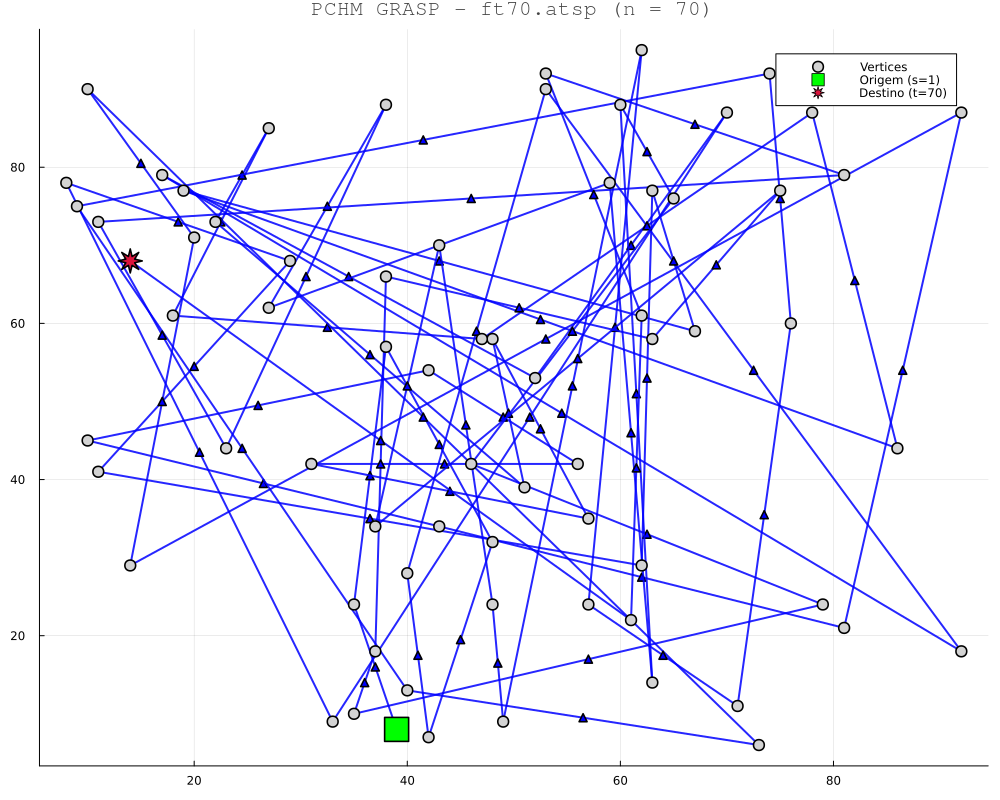
\includegraphics[width=\linewidth]{data/plots/ft70.png}
\caption{\texttt{ft70.atsp} ($n=70$, $Z_{\text{GRASP}} = 39608,00$)}
\end{minipage}
\end{figure}

\begin{figure}[H]
\centering
\begin{minipage}{0.48\textwidth}
\centering
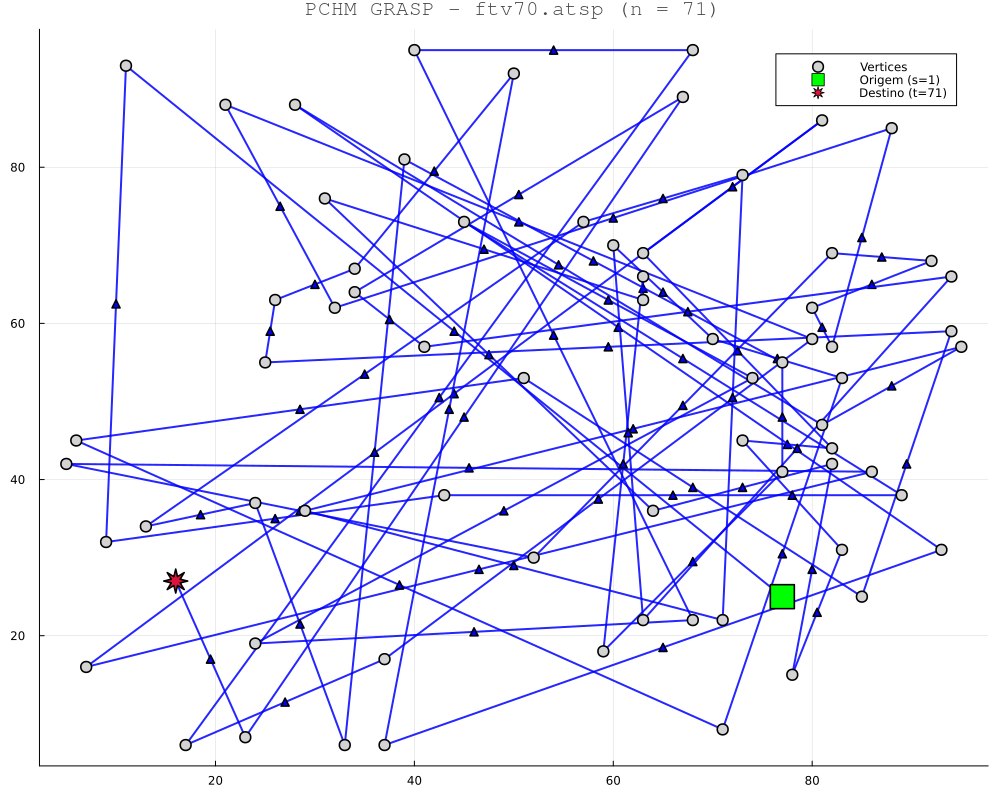
\includegraphics[width=\linewidth]{data/plots/ftv70.png}
\caption{\texttt{ftv70.atsp} ($n=71$, $Z_{\text{GRASP}} = 2104,00$)}\label{fig:ftv70}
\end{minipage}
\end{figure}

\section{Declaração de Uso de Inteligência Artificial (Atividade 3.1)}
Foi utilizada como apoio na estruturação e revisão do código das heurísticas, consulta sobre as vizinhanças de busca local (2-Opt, Or-Opt e Swap) e formatação deste relatório em \LaTeX.
\end{document}
